\documentclass{article}

% Language setting
% Replace `english' with e.g. `spanish' to change the document language
\usepackage[english]{babel}

% Set page size and margins
% Replace `letterpaper' with `a4paper' for UK/EU standard size
\usepackage[letterpaper,top=2cm,bottom=2cm,left=3cm,right=3cm,marginparwidth=1.75cm]{geometry}

% Useful packages
\usepackage[sorting=none]{biblatex}
\addbibresource{sample.bib} %Import the bibliography file
\usepackage{amsmath}
\usepackage{graphicx}
\usepackage{subcaption}
\usepackage[colorlinks=true, allcolors=blue]{hyperref}

\title{A Practical Project On Applying Forecasting Techniques For Power Consumption Prediction Using ARMA and ANNs}
\author{Mohammad Hossein Zolfagharnasab, \\
Safa Vakili}

\begin{document}
\maketitle

\begin{abstract}
Power consumption prediction is a critical requirement for governments and related organizations, as it plays a vital role in the strategic planning and management of energy resources nationally. Given its importance, the methodologies used for predicting power consumption are chosen with great care to guarantee accuracy and consistency. With the surge of studies in Artificial Intelligence (AI) in recent years, the area contributing to time-series forecasting has also received vivid enhancements \cite{ebrahimpour2011mixture}. In this regard, the current study is carried out to perform a comparative evaluation between the standard prediction models (such as ARMA, \& ARIMA) and  data-driven AI models particularly those employing Neural Networks. The dataset selected for this study is the \textbf{Practical Work 1} samples.\@
Based on the results, it can be observed that both models obtained a reasonable approximation of the prediction. However, the ANN approach found to be a more precise estimation.
\end{abstract}

\section{Introduction}
Accurate forecasting is essential for ensuring energy security, optimizing energy usage, and supporting economic development \cite{landsiedel2005accurate}. It allows policymakers to make informed decisions regarding infrastructure investments and energy policies that can sustain growth without overwhelming the grid \cite{salam2018comparison}.\@ Moreover, reliable power consumption predictions are critical for integrating renewable energy sources, as they help balance intermittent supplies with fluctuating demands \cite{ullah2019short}. This foresight is also vital for emergency preparedness and resilience planning, enabling authorities to anticipate and mitigate potential power shortages or disruptions. Ultimately, robust power consumption forecasting supports sustainable development goals by promoting efficient energy use and reducing environmental impacts, thereby contributing to a more stable and sustainable future \cite{ahn2022prediction}. Concerning the noted benefits, the current study is carried out to respond to the problems considered in \textbf{Practical work 1} that are:
\begin{itemize}
    \item Evaluating standard ARMA approach for predicting power consumption
    \item Developing models based on Neural Netwrok (NN) for predicting power consumption
    \item Comparing the accuracy and robustness of each technique
\end{itemize}

\section{Dataset}
The dataset used in this study comprised of a Comma-Separated-Value (CSV) file, which contains 1000 records that are labeled under \textit{ID}, and \textit{Y} value. As depicted in Figure \ref{fig:dataset}, it can be observed that the dataset has missing values after ID number 600.\\ 
In the current study, the first 600 records are considered as the train-set, and the remaining 400 values are considered the test-set, which are not exposed to the model during the training stage. Therefore, the model is subjected to regress the test-set and the specified missing values inside the test-set in order to conclude the prediction.

\begin{figure}
\centering
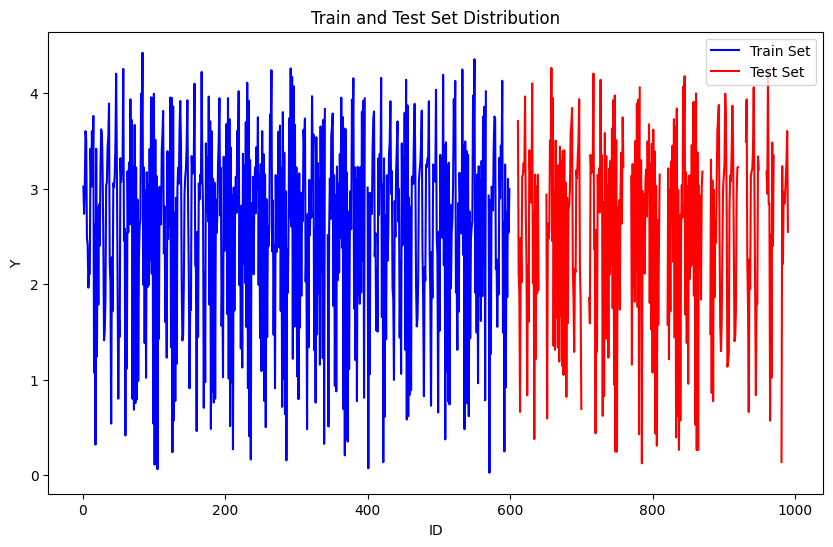
\includegraphics[width=0.8\linewidth]{Fig01.png}
\caption{\label{fig:dataset} Dataset used in this study.}
\end{figure}

\section{Background}
There are two models that have been evaluated in this study. First the Autoregressive Moving Average (ARMA) model is recognized as a pivotal statistical tool. Comprising both autoregressive (AR) and moving average (MA) components, the model is delineated by as below:
\begin{equation}
    ARMA(p, q) = \sum_{i=1}^p \phi_i X_{t-i} + \sum_{j=1}^q \theta_j \epsilon_{t-j} + \epsilon_t ,
\end{equation}
where \( \{X_t\} \) denotes the time-series, \( \{\epsilon_t\} \) are white noise error terms, \( \{\phi_i\} \) are coefficients for the AR terms, and \( \{\theta_j\} \) are coefficients for the MA terms. The variables \( p \) and \( q \) represent the order of the AR and MA components, respectively. 
Since ARMA is essentially a fixed model, selection of the  variables is generally guided by the Akaike Information Criterion (AIC) or the Bayesian Information Criterion (BIC), which assist in balancing model fit and complexity. In assessing the accuracy of the ARMA model, metrics such as the Mean Absolute Error (MAE), Root Mean Squared Error (RMSE), and Mean Absolute Percentage Error (MAPE) are also commonly employed to evaluate the model performance on the test samples. These metrics are integral for evaluating the predictive performance of the model, ensuring that the forecasts generated align closely with the observed data values.\\
Second, the Multilayer Perceptron (MLP) model, esteemed as a fundamental neural network architecture, is found as a robust and accurate asset for regression and general prediction. Characterized by its layered structure, the MLP consists of an input layer, one or more hidden layers, and an output layer. The model can be mathematically expressed through:
\begin{equation}
    y = f(W_n \dots f(W_2 f(W_1 x + b_1) + b_2) \dots + b_n),
\end{equation}
where \( x \) denotes the input vector, \( W_1, \dots, W_n \) are the weight matrices for each layer, \( b_1, \dots, b_n \) are the bias vectors, and \( f \) represents the activation function applied at each layer. Similar to ARMA, MLP requires a meticulous selection of hyper-parameters to achieve the highest performance. Consequently, the number of hidden layers, the number of neurons in each layer, and a the value corresponding to learning-rate and batch-size are the typical parameters that must be determined during the model development. Moreover, accuracy metrics such as Mean Squared Error (MSE), Root Mean Squared Error (RMSE), and Mean Absolute Error (MAE) are similarly utilized to evaluate the efficacy of MLP models in forecasting. It is also worth noting that MLPs may require extra measures such as cross-validation or sample normalization to prevent over-fitting and convergence difficulties.

\section{Proposed Method}
In the following, the solution process discussed earlier is explained in more details.
\subsection{ARMA workflow}
The ARMA procedure begins by determining the $p$ and $q$ variables corresponding to the MA and AR parts of the model. To do so, the Autocorrelation Function (ACF) and the Partial Autocorrelation Function (PACF) analysis are conducted which are both depicted in Figure \ref{fig:acf-pacf}.\\
The results reveal a gradual decrease (and alternation in sign) for the ACF, which suggests future values retain some correlation with past values across extended lags. The blue shaded area indicates the confidence interval, where  the Autocorrelations within are considered statistically insignificant, compared to those extending beyond this band.
\begin{figure} [h]
    \centering
    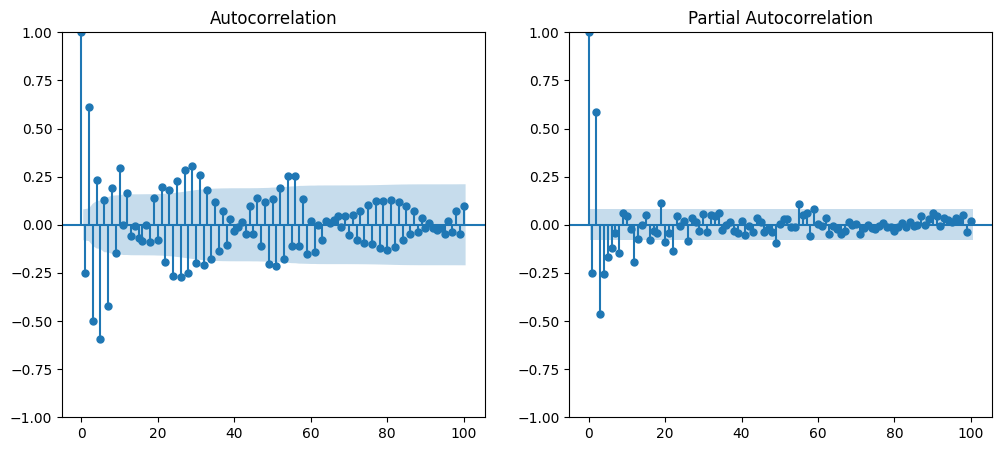
\includegraphics[width=\linewidth]{Fig02.png}
    \caption{\label{fig:acf-pacf} Results obtained from ACF and PACF analysis.}
\end{figure}

Next, the PACF plot on the right illustrates the correlation of the series with its lagged values. The plot displays a significant spike at lag 1, followed by autocorrelations that predominantly remain within the confidence interval, suggesting that an AR(1) component might be a strong candidate. The rapid decline in PACF after the initial lags (3 to 4) generally indicates the required number of autoregressive terms for an AR process.\\ 
As there are several options available for selecting $p$ and $q$ variables, this study performed a sensitivity analysis over a range of $p$ and $q$ parameters to determine the best hyper-parameters for the current scenario.\@ Furthermore, the Akaike Information Criterion (AIC) and the Bayesian Information Criterion (BIC) values were calculated per each pair to identify the promising candidates. Looking at the data in \ref{fig:sensitivity}, the choices can be summed up to three main options:
\begin{itemize}
    \item The lowest AIC: 1217.43 \& BIC: 1287.78 for (p=7, q=7).
    \item The AIC:1232.74 \& the lowest BIC value is 1285.50 for (p=8, q=2).
    \item A Balanced AIC: 1228.61 \& BIC: 1294.57, for (p=4, q=9).
\end{itemize}
AIC is focused more on the goodness of fit, potentially at the risk of overfitting. If the primary concern is finding the model that best explains the data without regard to the number of parameters as much, the AIC suggests using ARMA(7,7).
BIC includes a stronger penalty for the number of parameters, making it less prone to overfitting, especially in cases with larger data sets. Thus, If we are more concerned about overfitting and want a simpler model, the BIC suggests using ARMA(8,2).
Lastly, for a more balanced choice, we would ideally select a model with relatively low values for both AIC and BIC, and not necessarily the absolute lowest for either. This approach ensures a good balance between fit and simplicity, which can be obtained using ARMA (4, 9). In the current study, all three models were investigated.
\begin{figure}[h]
    \centering
    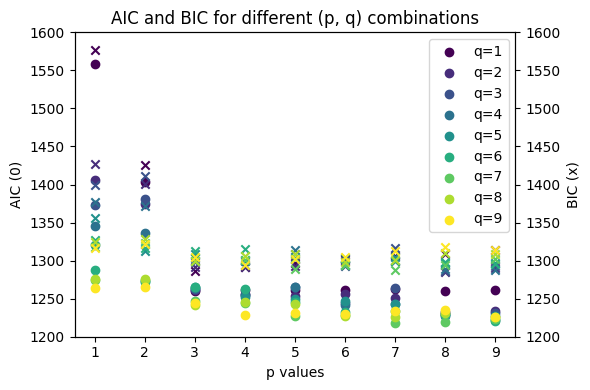
\includegraphics[width=0.75\linewidth]{Fig03.png}
    \caption{\label{fig:sensitivity} Sensitivity analysis over $p$ and $q$ variables.}
\end{figure}

\subsection{MLP workflow}
Utilizing the standard MLP for time-series forecasting is a more convenient approach compared with ARMA procedure, as the NN aims to reflect the time-series characteristic with the least effort in manual feature engineering, dataset evaluation, and statistical assumptions.\\
While following a similar train-test split, a standard normalization is carried out on the samples to increase the convergence. Next, the samples sequences are reduced into multiple chunks with a default window of 4. The window is a parameter similar to PACF, which promotes the impact of $Size_{W}$ variables into the model. Therefore, increasing the window size usually incorporates higher accuracy with a cost of computational time as well as implying more dependency.\\
Next, the MLP employed in this study consists of an input layer with window size, a hidden layer with 128 neurons, and an output layer. All the layers are also followed by a ReLU function. The size of each layer and activations are selected based on experimental evaluations. The model is trained using the Adam optimizer with a learning-rate of $0.001$, over 100 epochs. Also, the MSE loss function is utilized to evaluate the degree of fit as well as mitigating over-fitting.\\
Since the MLP implementation is a straight-forward procedure, we conclude the explanation of the workflow followed in this study.

\section{Results}
The results comprising the implemented models are depicted in Figure \ref{fig:ARMA}, \ref{fig:mlp}, and \ref{fig:ANN-AR}.\\
Beginning with ARMA family of models, Figure \ref{fig:ARMA} shows that all ARMA models were able to fit into the training set quite well. This demonstrates the potential of ARMA in understanding the general dynamics of a given time-series. However, all variations of the ARMA were unsuccessful to imitate the variations of the test set, and they were only capable of forecasting the average regime of the test samples.
Among the implemented ARMA models, ARMA(4,9) was found the most accurate to fit the training set with RMSE value of 1.019. Concerning that the other models contributed to the lowest AIC and BIC values, this observation confirms that the optimal pair of $p$ and $q$ must be determined by striking a balance between the AIC and BIC metrics. The RMSE value obtained by ARMA(4,9) for train-set was found 0.655, which was found slightly higher than ARMA(7,7). This concludes the predictions of ARMA model.\\
\begin{figure}[h!]
    \centering
    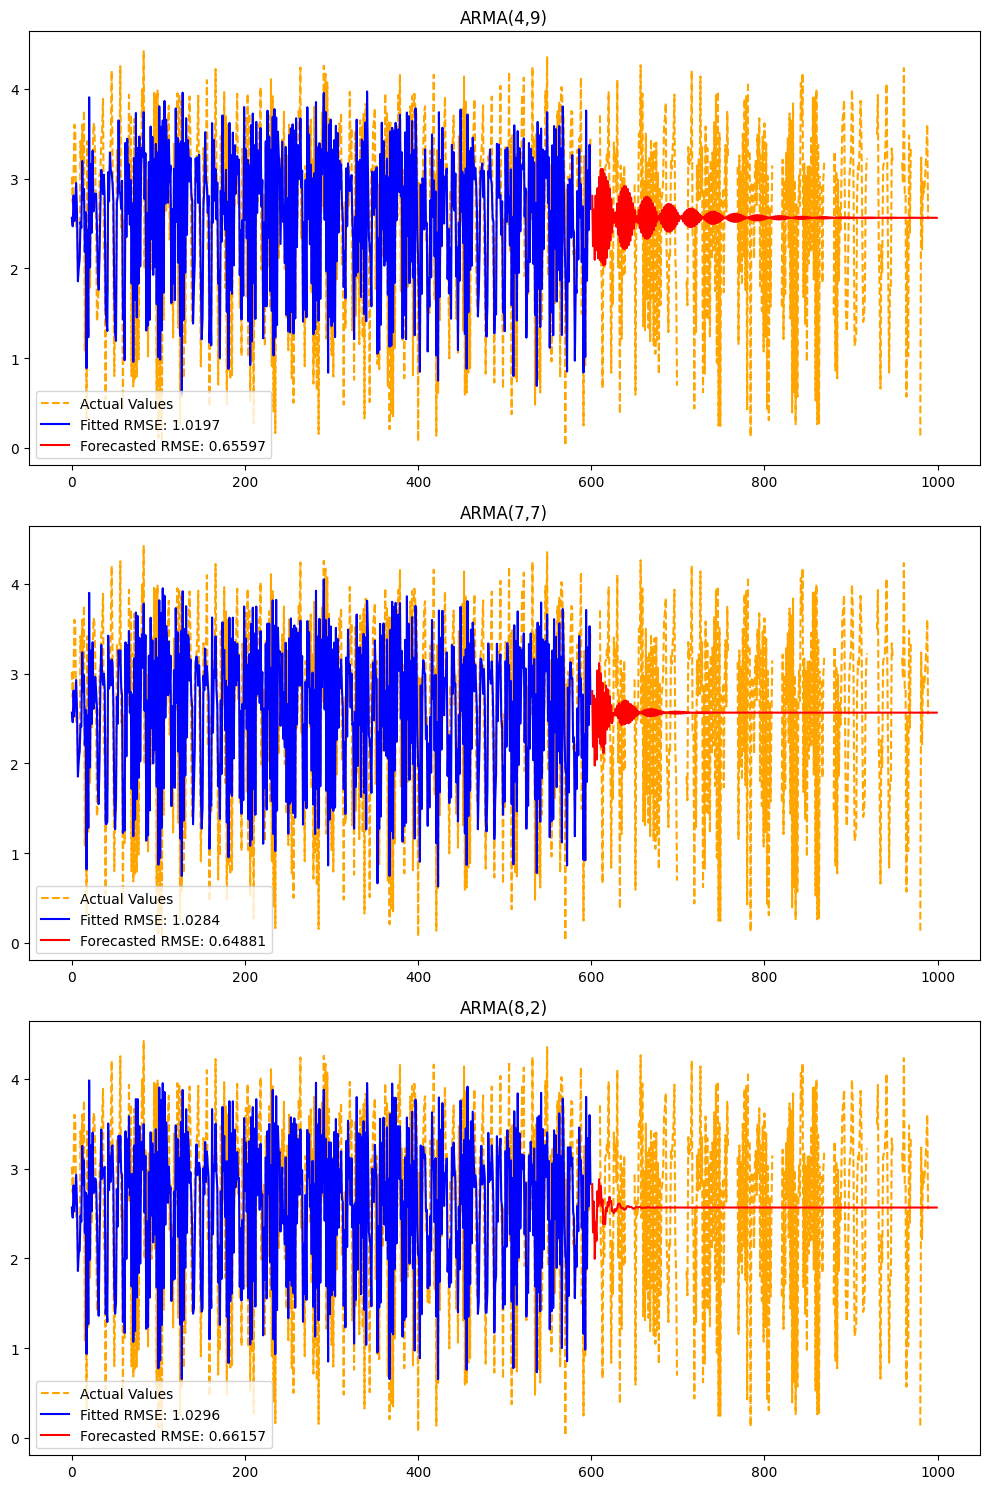
\includegraphics[width=0.75\linewidth]{Fig04.png}
    \caption{\label{fig:ARMA} ARMA predictions}
\end{figure}
\newpage
Next, we can observe the predictions of the MLP model in Figure \ref{fig:mlp}. Based on the results, a more accurate fit with RMSE value of 0.39 can be observed from the MLP model compared with the 1.02 RMSE value obtained ARMA variations. Concerning that a very shallow MLP model is utilized for the analysis, this proves the potential of MLP in understanding the hidden patterns reside in time-series.\\ 
Similarly, the results obtained by the MLP in the test-set was found even more promising as the MLP was capable of imitating the oscillations of the test-set quite well. Based on the results, a window size of 4 was sufficiently accurate for the model to forecast the future sequences. The RMSE obtained in the testset was also found 0.29, which was two times better than the the 0.65 value acquired by the ARMA model.
\begin{figure}[h!]
    \centering
    \begin{subfigure}{0.675\linewidth}
        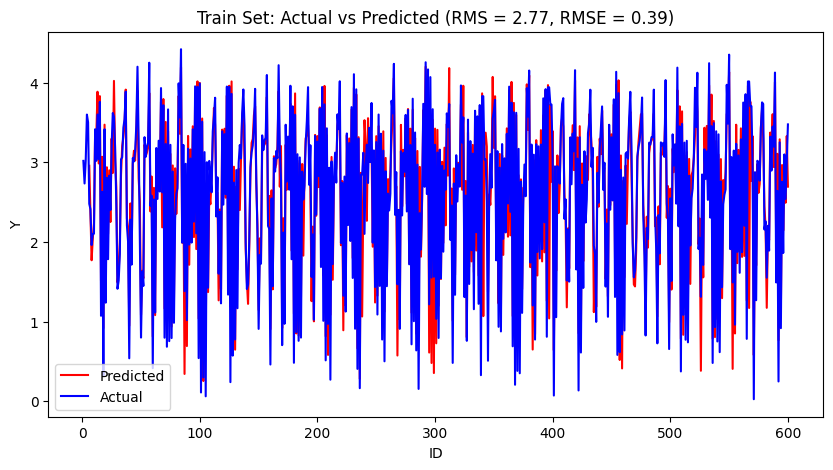
\includegraphics[width=\linewidth]{Fig05-1.png}
        \label{fig:05A}
    \end{subfigure}
    % \vspace{1cm} % Adds vertical space between the images
    \begin{subfigure}{0.675\linewidth}
        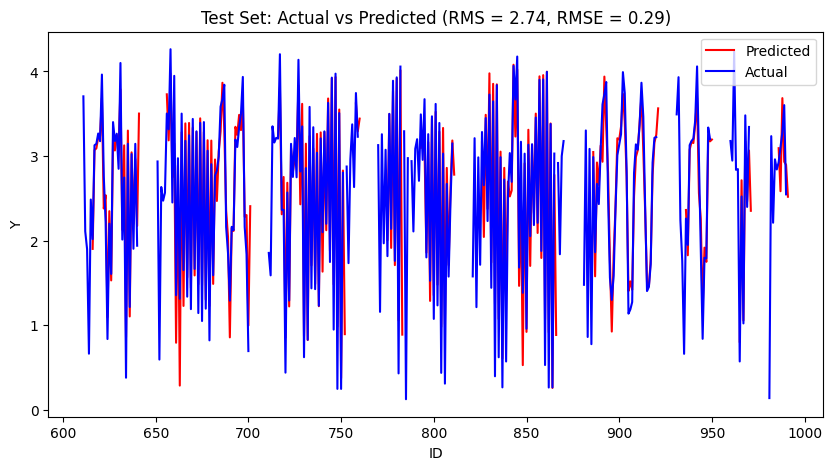
\includegraphics[width=\linewidth]{Fig05-2.png}
        \label{fig:05B}
    \end{subfigure}
    \caption{MLP predictions}
    \label{fig:mlp}
\end{figure}
\newpage
As the MLP model was successfully in predicting the future sequences, the current study carried out a final analysis to examine the auto-regressive nature of this method. To do so, only the initial sequence of time-series (the first 4 elements of the training-set) was exposed to the model and the model was tasked to auto-regressively predict all the future sequences up to the end of the test-set. As depicted in Figure \ref{fig:ANN-AR}, the model has successfully imitate both patterns of train and test sets with the RMSE value of 0.34. This concludes the analysis over the MLP model.
\begin{figure}[h!]
    \centering
    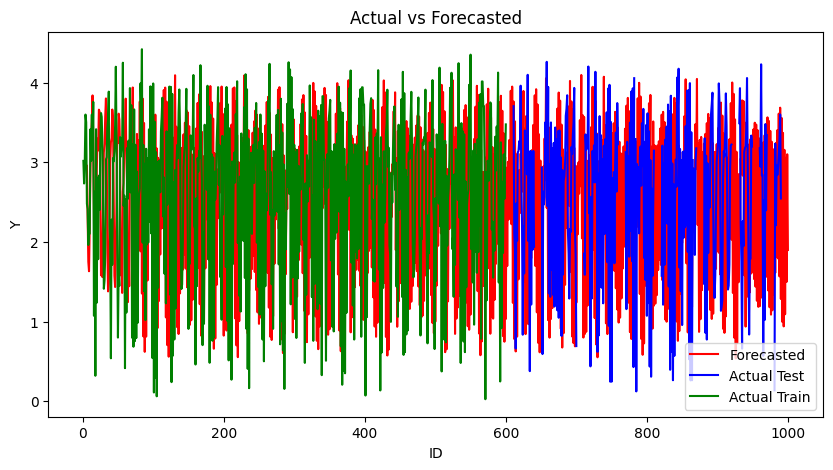
\includegraphics[width=0.675\linewidth]{Fig06.png}
    \caption{\label{fig:ANN-AR} Auto-Regressive MLP prediction}
\end{figure}

\newpage
\section{Future works}
There are two directions that the current work can be proceeded. First, the current work could be progressed by applying other variations of ANN such as Recurrent Neural Networks (RNNs), and transformers to evaluate the potential of these models for short-term to long-term predictions.\\
Second, the current work can be continued by analysing the sensitivity of MLP models on the solution parameters and the time-series elements. Such interoperability analysis can be used later as feed-back points to improve the models.

\section{Conclusion}
This study has conducted a comparison between traditional statistical methods and modern neural network approaches for forecasting power consumption. Our analysis revealed that while ARMA models provide a robust baseline, they struggle to capture complex patterns in data, especially in the test set. In contrast, the MLP model, with its capability to model nonlinear relationships, outperformed the ARMA models.\\
The findings from the ARMA models highlighted the importance of selecting appropriate \(p\) and \(q\) parameters, where a balance between AIC and BIC metrics was essential to optimize model performance without overfitting. The superior performance of the MLP model underscores the potential of neural networks in time-series forecasting, providing a more accurate and adaptable tool for predicting power consumption.
Furthermore, the ability of the MLP to auto-regressively predict future sequences using minimal initial data demonstrates its effectiveness in real-time or long-term forecasting applications. This capability is particularly relevant for power grid management and planning, where timely and accurate forecasts are crucial.

\printbibliography %Prints bibliography


\end{document}